\documentclass[floatsintext,doc]{apa6}
\usepackage{lmodern}
\usepackage{amssymb,amsmath}
\usepackage{ifxetex,ifluatex}
\usepackage{apacite}
%\usepackage{hyperref}
\usepackage[utf8]{inputenc}
%\usepackage{fourier}%
%\usepackage{fourier}%
%\usepackage{heuristica}
\usepackage{geometry}

\usepackage{array}
\usepackage{tabularx}
\usepackage{caption}

\usepackage{fixltx2e} % provides \textsubscript
\ifnum 0\ifxetex 1\fi\ifluatex 1\fi=0 % if pdftex
  \usepackage[T1]{fontenc}
  \usepackage[utf8]{inputenc}
\else % if luatex or xelatex
  \ifxetex
    \usepackage{mathspec}
  \else
    \usepackage{fontspec}
  \fi
  \defaultfontfeatures{Ligatures=TeX,Scale=MatchLowercase}
\fi
% use upquote if available, for straight quotes in verbatim environments
\IfFileExists{upquote.sty}{\usepackage{upquote}}{}
% use microtype if available
\IfFileExists{microtype.sty}{%
\usepackage{microtype}
\UseMicrotypeSet[protrusion]{basicmath} % disable protrusion for tt fonts
}{}

%\hypersetup{unicode=true,
%            pdftitle={Not unreasonable: Uncertainty in the language of logic},
%            pdfauthor={Michael Henry Tessler~\& Michael Franke},
%            pdfkeywords={semantics; pragmatics; negation; Bayesian cognitive model; Rational Speech Act},
%            pdfborder={0 0 0},
%            breaklinks=true}
%\urlstyle{same}  % don't use monospace font for urls
\usepackage{graphicx,grffile}
\makeatletter
\def\maxwidth{\ifdim\Gin@nat@width>\linewidth\linewidth\else\Gin@nat@width\fi}
\def\maxheight{\ifdim\Gin@nat@height>\textheight\textheight\else\Gin@nat@height\fi}
\makeatother
% Scale images if necessary, so that they will not overflow the page
% margins by default, and it is still possible to overwrite the defaults
% using explicit options in \includegraphics[width, height, ...]{}
\setkeys{Gin}{width=\maxwidth,height=\maxheight,keepaspectratio}
\IfFileExists{parskip.sty}{%
\usepackage{parskip}
}{% else
\setlength{\parindent}{0pt}
\setlength{\parskip}{6pt plus 2pt minus 1pt}
}
\setlength{\emergencystretch}{3em}  % prevent overfull lines
\providecommand{\tightlist}{%
  \setlength{\itemsep}{0pt}\setlength{\parskip}{0pt}}
\setcounter{secnumdepth}{0}
% Redefines (sub)paragraphs to behave more like sections
\ifx\paragraph\undefined\else
\let\oldparagraph\paragraph
\renewcommand{\paragraph}[1]{\oldparagraph{#1}\mbox{}}
\fi
\ifx\subparagraph\undefined\else
\let\oldsubparagraph\subparagraph
\renewcommand{\subparagraph}[1]{\oldsubparagraph{#1}\mbox{}}
\fi

%%% Use protect on footnotes to avoid problems with footnotes in titles
\let\rmarkdownfootnote\footnote%
\def\footnote{\protect\rmarkdownfootnote}



% these packages are needed to insert results 
% obtained from R into the LaTeX document
\usepackage{pgfplotstable}
\usepackage{csvsimple}
\usepackage{siunitx}

% set the name of the folder in which the CSV files with 
% information from R is stored
\newcommand{\datafoldername}{csv_data_4_tex}

% the following code defines the convenience functions
% as described in the main text below

% rlgetvalue returns whatever is the in cell of the CSV file
% be it string or number; it does not format anything
\newcommand{\rlgetvalue}[4]{\csvreader[filter strcmp={\mykey}{#3},
             late after line = {{,}\ }, late after last line = {{}}]
            {\datafoldername/#1}{#2=\mykey,#4=\myvalue}{\myvalue}}

% rlgetvariable is a shortcut for a specific CSV file (myvars.csv) in which
% individual variables that do not belong to a larger chunk can be stored
\newcommand{\rlgetvariable}[1]{\csvreader[]{\datafoldername/myvars.csv}{#1=\myvar}{\myvar}\xspace}

% rlnum format a decimal number
\newcommand{\rlnum}[2]{\num[output-decimal-marker={.},
                             exponent-product = \cdot,
                             round-mode=places,
                             round-precision=#2,
                             group-digits=false]{#1}}

\newcommand{\rlnumsci}[2]{\num[output-decimal-marker={.},
                          scientific-notation = true,
                             exponent-product = \cdot,
                             round-mode=places,
                             round-precision=#2,
                             group-digits=false]{#1}}

\newcommand{\rlgetnum}[5]{\csvreader[filter strcmp={\mykey}{#3},
             late after line = {{,}\ }, late after last line = {{}}]
            {\datafoldername/#1}{#2=\mykey,#4=\myvalue}{\rlnum{\myvalue}{#5}}}

\newcommand{\rlgetnumsci}[5]{\csvreader[filter strcmp={\mykey}{#3},
             late after line = {{,}\ }, late after last line = {{}}]
            {\datafoldername/#1}{#2=\mykey,#4=\myvalue}{\rlnumsci{\myvalue}{#5}}}






%  \title{Not unreasonable: Uncertainty in the language of negation}
%  \title{Not unreasonable: Multiple opposite meanings are entertained when understanding negation}
%\title{Not stating the opposite: Double negations result in nonredundant meanings}
\title{Supplementary Information: Two negatives don't exactly make a positive}
    \author{Michael Henry Tessler\textsuperscript{1}~\& Michael Franke\textsuperscript{2}}
    \date{}
  
\shorttitle{SOM-R: Uncertain logical language}
\affiliation{
\vspace{0.5cm}
\textsuperscript{1} Massachusetts Institute of Technology\\\textsuperscript{2} University of Osnabr\"{u}ck}
\keywords{}
\usepackage{csquotes}
\usepackage{upgreek}
\captionsetup{font=singlespacing,justification=justified}

\usepackage{longtable}
\usepackage{lscape}
\usepackage{multirow}
\usepackage{tabularx}
\usepackage[flushleft]{threeparttable}
\usepackage{threeparttablex}

%\newenvironment{lltable}{\begin{landscape}\begin{center}\begin{ThreePartTable}}{\end{ThreePartTable}\end{center}\end{landscape}}

\makeatletter
\newcommand\LastLTentrywidth{1em}
\newlength\longtablewidth
\setlength{\longtablewidth}{1in}
\newcommand{\getlongtablewidth}{\begingroup \ifcsname LT@\roman{LT@tables}\endcsname \global\longtablewidth=0pt \renewcommand{\LT@entry}[2]{\global\advance\longtablewidth by ##2\relax\gdef\LastLTentrywidth{##2}}\@nameuse{LT@\roman{LT@tables}} \fi \endgroup}


%\DeclareDelayedFloatFlavor{ThreePartTable}{table}
%\DeclareDelayedFloatFlavor{lltable}{table}
%\DeclareDelayedFloatFlavor*{longtable}{table}
\makeatletter
%\renewcommand{\efloat@iwrite}[1]{\immediate\expandafter\protected@write\csname efloat@post#1\endcsname{}}
\makeatother
\usepackage{tabularx}
\usepackage{multicol}
\usepackage{wrapfig}
\usepackage{gensymb}
\usepackage{tikz}
\usepackage{caption}
\usepackage{booktabs}
\usepackage{xcolor}

\begin{document}
\maketitle

\newcommand*\diff{\mathop{}\!\mathrm{d}}
\newcommand{\denote}[1]{\mbox{ $[\![ #1 ]\!]$}}
\newcommand{\tableref}[1]{Table$\thinspace$\ref{#1}}
\newcommand{\figref}[1]{Fig.$\thinspace$\ref{#1}}
\newcommand{\appref}[1]{Appendix \ref{#1}}
\newcommand{\sectionref}[1]{Section \ref{#1}}
\definecolor{Red}{RGB}{255,0,0}
\definecolor{Green}{RGB}{10,200,100}
\definecolor{Blue}{RGB}{10,100,200}
\definecolor{grey}{RGB}{40,40,40}

\newcommand{\red}[1]{\textcolor{Red}{#1}}  
\newcommand{\mf}[1]{\textcolor{Green}{[mf: #1]}}  
\newcommand{\mht}[1]{\textcolor{Blue}{[mht: #1]}}

%\newcommand{\wrapmf}[1]{#1}

\providecommand{\tightlist}{%
  \setlength{\itemsep}{0pt}\setlength{\parskip}{0pt}}


Here we describe the details of the computational models used to generate the predictions for the various hypotheses (\emph{Aristotle}, \emph{George Orwell}, \emph{Uncertain negation}) in the paper.


\section{Computational Modeling Details}

%Negation is the semantic operation of forming an opposite, but there is more than one way to convey an opposite. 

%Formally, a contradictory opposition turns predicate $H$ into $\neg H$; contrary opposition turns $H$ into $\tilde{H}$. 
%Contradictory opposition can be iterated ($\neg \neg H$) as in the intended meaning behind ``the enemy of my enemy is my friend''; standard logic does not allow for the iteration of contrary opposition (i.e., $\tilde{\tilde{H}}$ is not a logical possibility;  \citeNP{Horn1989:Natural}).
%


% \(\neg \neg happy\) 
%The opposite of $(x > \theta_1)$ is either $(x \leq \theta_1)$ or $(x < \theta_2)$.
%.\footnote{
%Another example of iterated contradictory meaning is the intended meaning behind ``the enemy of my enemy is my friend''.
%} 
%With these basic facts, we provide an informal description of our model before moving onto its formal characterization.
 %\red{(e.g., there is no unshort)}.\% \cite{Horn1989:Natural}.
%QAs a result, a single negative (\enquote{not happy} and \enquote{unhappy}) can mean either \(\neg happy\) or \(\tilde{happy}\), while double negatives (\enquote{not unhappy}) may mean \(\neg \neg happy\) or \(\neg \tilde{happy}\) (Fig.\(\thinspace\)\ref{fig:lexicon-model}).}

Our primary hypothesis is that the logical distinction between contradictory~vs.~contrary opposition manifests in natural language markers (\enquote{not}, \enquote{un-}) in an uncertain way. % and that  listeners maintain uncertainty about the mapping between logical negations and natural language negation% (\enquote{not}, \enquote{un-}) in a stable, context-invariant manner. 
%We imagine and resolve their uncertainty in context.  
A listener who hears statements involving negation reasons over a hypothesis space of possibilities about the mappings between natural language negation markers  (\enquote{not}, \enquote{un-}) and the negation operations of contradictory and contrary opposition.
\emph{Contradictory} opposites cannot both be true and they cannot both be false, such as an integer being either even or odd (\emph{even} and \emph{odd} are contradictions).
\emph{Contrary} opposites cannot both be true but they can both be false: A person could be neither tall nor short (\emph{tall} and \emph{short} are contraries). 
Formally, a contradictory opposition turns a predicate $H$ into $\neg H$, and contradictory opposition can be iterated ($\neg \neg H$; e.g., \emph{the enemy of my enemy is my friend}).
Contrary opposition turns $H$ into a new predicate $\tilde{H}$, but standard logic does not allow for the iteration of contrary opposition (i.e., $\tilde{\tilde{H}}$ is not a logical possibility;  \citeNP{Horn1989:Natural}).
%The hypothesis space of meanings is constrained by those definitions.
%Because contraries do not iterate, a double negative like \emph{not unhappy} could convey a double contradiction ($\neg \neg H$) or a contradiction about a contrary ($\neg \tilde{H}$): The former carries the same meaning as $H$ (\emph{happy}) whereas the latter conveys a distinct meaning. 
%Intuitively, a rational speaker whose goal is to convey $H$ (or, $\neg \neg H$) would avoid the double negative construction because it is more verbose; thus, a sophisticated listener could backwards infer that a speaker who uses a double negative means to convey the expression with a unique meaning: $\neg \tilde{H}$.
%This uncertain negation hypothesis further predicts that \emph{not happy} and \emph{unhappy} inherit the same set of possible meanings; \emph{a priori} it is not obvious whether the two expressions mean something distinct from one another. 
%\mht{he}
%This hypothesis further predicts that a listener who hears only a single adjective phrase in isolation (e.g., \enquote{unhappy}) has no basis from which to decide whether a contrary or contradiction was intended, and thus the listener should impart no meaning difference between an isolated .
%and thus a rational speaker would not have bothered to say \emph{not unhappy} (a more complex expression) if a double contradiction was their intention, so they likely were contradicting a contrary.

%This mutual-exclusivity kind of reasoning is also predicted to occur were a speaker to use two distinct negations in the same context (e.g., \enquote{Jones is not happy, while Smith is unhappy}, also Krifka's example above); that is, the model predicts that \emph{unhappy} is intended to convey more negative feelings than \emph{not happy} when the model observes the speaker using both kinds of negation in the same context.
%Thus, hearing a double negation does provide sufficient evidence to the listener that the speaker intends two different kinds of negation. 
%\mht{do we want to say here that we are looking at the negation of scalar adjectives, as opposed to other negation like phenomena?}
%Then, interpreting negated antonyms of scalar adjectives like \enquote{not unhappy} involves not only reasoning about negation but how various kinds of negation interact with the vagueness of scalar adjectives like \emph{happy} or \emph{tall}.


%\begin{figure}[h]
%\centering 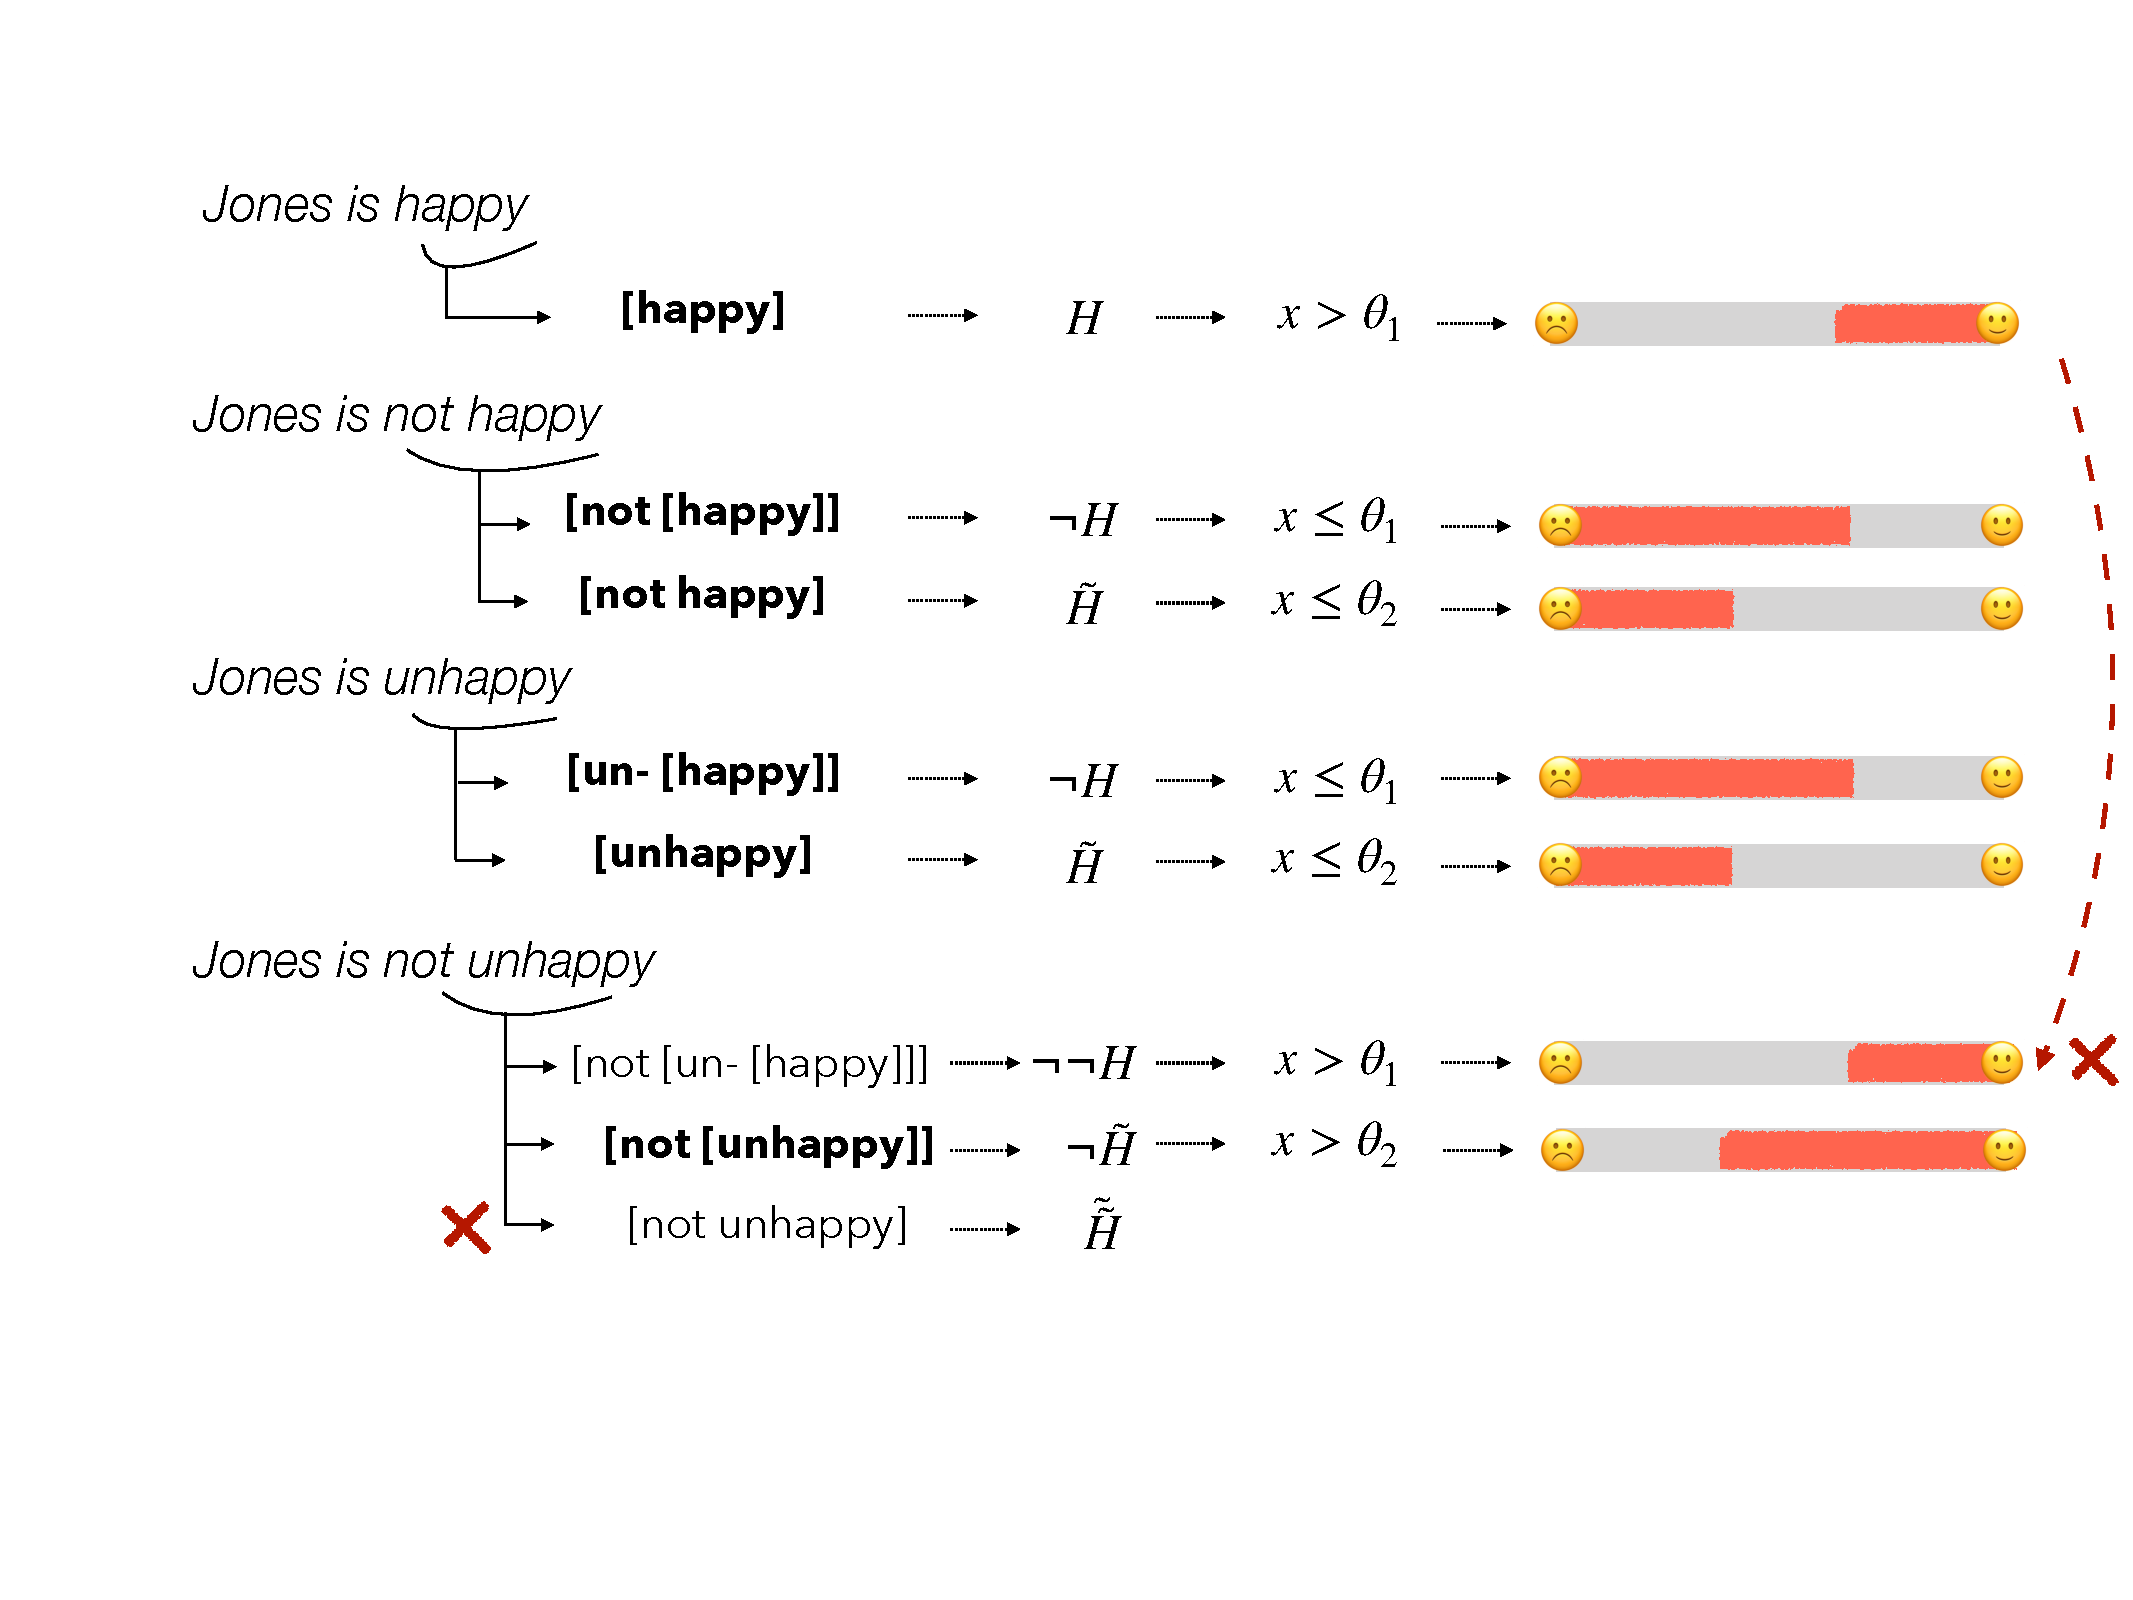
\includegraphics[width=0.8\textwidth]{figs/schematicMeanings}  
%\caption{Set of possible meanings for antonym pairs and their negations for the uncertain negation model. 
%Both ``not happy'' and ``unhappy'' could signal either contradictory $\neg H$ or contrary $\tilde{H}$ negation.
%``Not unhappy'' can signal a double contradiction  $\neg \neg H$  or a contradiction of a contrary  $ \neg \tilde{H}$. A double contrary $\tilde{\tilde{H}}$ is not logically possible. A double contradiction  $\neg \neg H$  is pragmatically unlikely, because the same meaning is expressed by just the simple positive $H$. Scales on the right denote hypothetical interpretations of the different meanings.}
%\label{fig:meanings}
%\end{figure}

%\mht{can we model this as an L2, where Lassiter adj model is modularized into $P(x \mid u, \mathcal{L})$ and we don't need to talk about thresholds?}
%\begin{align}
%P_L(x, \mathcal{L} \mid u) &\propto P_S(u \mid x, \mathcal{L}) \cdot P(x) \cdot P(\mathcal{L}) \\
%P_S(u \mid x, \mathcal{L}) &\propto \exp{(\alpha \cdot \ln {P(x \mid u, \mathcal{L})} - \text{cost}(u))} \label{eq:S1}
%\end{align}


%We hypothesize that \emph{lexical uncertainty}---uncertainty in the meaning of words---pervades even the language of logical devices, which interacts with conversational reasoning to give rise to a panoply of context-specific interpretations.
%Specifically, we posit that overt negation markers (\enquote{not}, \enquote{un-}) can convey different kinds of negation and that listeners resolve their uncertainty about the meaning in context.

We formalize this logic in a computational model drawing on the tools of formal semantics and probabilistic models of pragmatics \cite{Franke2015a, Goodman2016:RSA}. 
This formal model allows us to interrogate the conditions under which the above logic actually results in the interpretations we posit.
%; it also allows us to understand the contribution of the vagueness of predicates like \enquote{happy} or \enquote{tall} (i.e., that there is no single threshold beyond which a person qualifies as tall). 
Formally, a scalar adjective (e.g., \enquote{happy} or $H$) is thought to be literally true when the degree associated with that adjective \(x\) (e.g., the degree of happiness) is greater than some contextually-determined threshold \(\theta_1\): \(\mbox{ $[\![H]\!]$}(x, \theta_1): x > \theta_1\) \cite{Kennedy2007}.
The intuition for this semantic representations comes from adjectives like \emph{tall}, where the underlying dimension is relatively transparent (height) and the contextually-determined threshold allows for context-sensitive interpretations (a tall boy vs. a tall building).
%If a negation marker (e.g., \enquote{not}) creates a 

The contradictory opposite of such a meaning is simply that the degree is less than or equal to that same threshold: \( \mbox{ $[\![\neg H]\!]$}(x, \theta_1): x \leq \theta_1\).
The contrary opposite, on the other hand, creates a new predicate, which for a gradable adjective takes the form of a function with its own, distinct threshold \(\theta_2\): \(\mbox{ $[\![ \tilde{H} ]\!]$}(x, \theta_2): x < \theta_2\).
% which can in principle receive a different value than threshold $\theta_1$ for the positive adjective
If listeners are uncertain about how \enquote{not} and \enquote{un-} map onto these logical meanings, then negated positives like \enquote{not happy} and morphological antonyms like \enquote{unhappy} could in principle take either meaning. 
The hypothesis space of meanings for negated antonyms like \enquote{not unhappy} is constrained by the fact that contraries do not iterate; thus, negated antonyms either correspond to a double application of contradictory negation or a contradiction of a contrary.\footnote{``not un-H'' can then be either \(\neg \neg H\) or \(\neg (\tilde{H})\). Cashing these meanings out in terms of scalar adjectives, the order of operations need not matter: \(\neg (\tilde{H})\) $= \tilde{(\neg H)}$ , because both imply two sign-changes and one tokenization of a new threshold.}




%The act of producing a negated antonym (\enquote{not unhappy}) can then act as a signal towards the kinds of oppositions that the speaker had in mind (e.g., that the speaker intends to convey a contradictory negation of a contrary opposite).
%\mht{i think this point could be moved to a model implementation appendix or footnote}

%\red{Contradictory opposition can be iterated (\(\neg \neg Hx\)) but contrary opposition cannot \cite{Horn1989:Natural}.
%As a result, a single negative (\enquote{not happy} and \enquote{unhappy}) can mean either \(\neg happy\) or \(\tilde{happy}\), while double negatives (\enquote{not unhappy}) may mean \(\neg \neg happy\) or \(\neg \tilde{happy}\) (Fig.\(\thinspace\)\ref{fig:lexicon-model}).}

%In order to generate predictions, 
We embed these literal meanings in a probabilistic model of pragmatic reasoning, wherein a pragmatic listener $L_1$ resolves the meaning of an utterance $u$ by reasoning about why a rational speaker $S_1$ would have bothered to produce said utterance.
Eqs.~\ref{eq:L0}--\ref{eq:L1} describe a recursive Bayesian model in the Rational Speech Act tradition \cite{Franke2015a, Goodman2016:RSA}, in which the listener  has additional uncertainty about how their interlocutor (speaker $S_1$) uses negation markers to convey contradictory~vs.~contrary negations \cite{Bergen2016}.
We additionally take into account the vagueness of scalar adjectives using the technique proposed by \citeA{Lassiter2015} to derive thresholds \(\theta\) for interpreting vague adjectives (e.g., happy) in context:

%We formalize this as a prior distribution over possible lexica for the speaker $P(\mathcal{L})$.
%This model also takes into account the fact the scalar adjectives like \emph{happy} or \emph{tall} exhibit vagueness; i.e., there is no single, fixed $\theta$ beyond which the adjective is true. 
%---couched i---also a recursive reasoning model wherein a pragmatic listener \(L_{1}\) tries to resolve the intended meaning of an utterance \(u\) (e.g., \enquote{Jones is not unhappy}) by combining its prior beliefs about the degree of Jones' happiness \(P(x)\) with the Gricean assumption that speakers are generally cooperative \(S_1\) (Eqs.\(\thinspace\)\ref{eq:L1}-\ref{eq:L0}):
%Listener uncertainty about the interpretation of negation markers is modeled as uncertainty about the speaker's lexicon \(\mathcal{L}\) \cite{Bergen2016}.

\vspace*{-0.5cm}

\begin{align}
L_{0}(x \mid u, \theta, \mathcal{L}) &\propto \mathcal{L}(u, x, \theta) \cdot P(x) \label{eq:L0} \\
S_{1}(u \mid x, \theta, \mathcal{L}) &\propto \exp{(\alpha \cdot \ln {L_{0}(x \mid u, \theta, \mathcal{L})} - \text{cost}(u))} \label{eq:S1}\\
L_{1}(x, \theta, \mathcal{L} \mid u) &\propto S_{1}(u \mid x, \theta, \mathcal{L}) \cdot P(x) \cdot  P(\theta) \cdot P(\mathcal{L}) \label{eq:L1}
\end{align}

The literal listener \(L_0\) (Eq. \ref{eq:L0}) updates their prior beliefs over the degree \(P(x)\) via an utterance's literal meaning in lexicon \(\mathcal{L}\),
where \(\mathcal{L}(u, x, \theta)\) gives the truth-value of the utterance \(u\) in lexicon \(\mathcal{L}\) when applied to degree \(x\) (e.g., for $u= $\enquote{happy}, $\mathcal{L}$ returns a 1 when $x>\theta$ and a 0 when  $x\leq\theta$).
The representation of prior beliefs $P(x)$ encodes prior expectations about the degree (e.g., how happy people are likely to be), which we assume for simplicity to be a uniform distribution. 
The speaker (Eq.~\ref{eq:S1}) is a soft-max rational agent (with degree of rationality  $\alpha$) who aims to act in accordance with a standard, information-theoretic utility function that tracks how well an utterance conveys the speaker's intended meaning $x$ (i.e., the degree of happiness) to this literal listener---$\ln {L_{0}(x \mid u, \theta, \mathcal{L}}$)---while taking into account the cost of the utterance---$\text{cost}(u)$.
We assume that negation created by morphology (e.g., ``un-'' + happy) adds cost to the utterance as does creating a negation using the particle ``not'', and that the cost of ``un-'' is less than the cost of ``not''.\footnote{The uncertain negation model's qualitative predictions are sensitive to the exact values of the parameters. The predictions we show are invariant to cost so long as $\text{cost}(un) \leq \text{cost}(not)$ and $\alpha$ is relatively small. Our goal is to show, under intuitively plausible parameter values consistent with the literature using Rational Speech Act models, the uncertain negation model has the capacity to the make the predictions we describe; none of the alternative models we articulate have the capacity to make the unique predictions of the uncertain negation model.}
The intended meaning in this model is the value along a dimension referenced by an adjective (e.g., a degree of happiness).\footnote{
	This meaning is a special case of modeling meaning as a probability distribution over degrees of happiness (e.g., the speaker has only a rough sense of their personal degree of happiness), in which case the speaker's utility would be a function of the KL divergence between the literal listener's prior and posterior distributions over the degree given the utterance. 
}
The pragmatic listener (Eq.~\ref{eq:L1}) interprets an utterance by reasoning about three variables: the intended meaning or degree $x$, the threshold beyond which a scalar adjective is literally true  $\theta$, and the speaker's lexicon \(\mathcal{L}\) describing how the speaker uses negation. 
%, and the likelihood \(S_1(u \mid x, \theta, \mathcal{L})\) that a cooperative information-maximizing speaker would utter the adjective given a degree \(x\), threshold \(\theta\), and lexicon \(\mathcal{L}\).
%The speaker model \(S_1\) (Eq.\ref{eq:S1}) describes an approximately rational agent (with degree of rationality \(\alpha\)) trying to inform a naive listener \(L_0\) about the degree \(x\).


%\begin{figure}
%\centering
%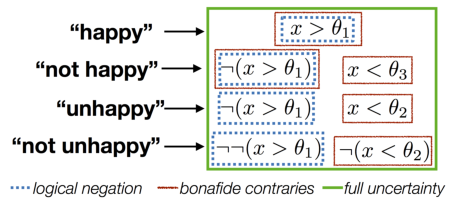
\includegraphics{figs/lexicon-model-1.pdf}
%\caption{\label{fig:lexicon-model}Space of possible meanings in the lexicon prior for the \emph{logical negation}, \emph{bonafide contraries}, and the full \emph{uncertain negation} models.}
%\end{figure}



In the main text, we compare the predictions of this uncertain negation model to two theoretically-interesting alternative models: one in which negation markers only map onto contradictory negation (the \emph{George Orwell} hypothesis) and one in which ``un-'' denotes contrary negation while ``not'' denotes contradictory negation (the \emph{Aristotle} hypothesis). 
Both of these models plus the uncertain negation model presented in the main text incorporate vagueness into the meaning of the adjective (i.e., adjectives mean that the degree of happiness of greater than some threshold $\theta$ which is inferred by the listener).
Here, we additionally compare these models to two other simpler alternatives in which there is no vagueness about the meaning of the adjective. 
First, we compare to a ``Vanilla RSA'' model which has neither lexical uncertainty about negation nor vagueness in the meaning of the adjective \cite{Frank2012}; we assume for this model an Aristotelean analysis of the negation markers (``not'' means contradiction; ``un-'' means contrary) operating over fixed threshold meanings: \enquote{happy} means \(>70\%\) on the happiness scale; \enquote{unhappy} means \(<30\%\).
We call this model \emph{Aristotle no vagueness}.
Second, we compare to an uncertain negation model without vagueness. 
This model has the same fixed threshold meanings for the adjectival utterances but has uncertainty as to whether or not ``un'' and ``not'' convey contradictory~vs.~contrary negation. 
We omit the predictions of the logically possible \emph{George Orwell} (no vagueness) model, because they are not qualitatively different from the model with vagueness.
%Second, we compare to the Vague RSA model of \citeA{Lassiter2015}, assuming that all negation markers entail contradictory negation (the \emph{logical negation} or \emph{George Orwell} model).
%Finally, we construct a \emph{bonafide contraries} model, building on \citeA{Lassiter2015}'s Vague RSA model by assuming morphological antonyms (\emph{un-}) convey contrary negation (e.g., \emph{unhappy} is to \emph{happy} how \emph{short} is to \emph{tall}) while the negation particular \emph{not} conveys contradictory negation.
%Finally, we construct fixed-threshold version of the Uncertain Negation model: this model is a lexical uncertainty model in the style of \citeA{Bergen2016}, which differs from our Uncertain Negation model only in its treatment of the semantics of the adjective as fixed as opposed to vague. 

\begin{table}[t]
\centering
\begingroup\fontsize{10pt}{11pt}\selectfont
\begin{tabularx}{0.9\textwidth}{l|c|c|c}
\toprule
Model Name                      & “happy”        & “un-”                            & “not ”                           \\ \midrule% & Description\\ \midrule
Aristotle no Vagueness                                                    & $x > 0.7$      & $x < 0.3$                        & $x < 0.7$                        \\% & Hard-coded contraries and contradictions \\
Aristotle with Vagueness                                 & $x > \theta_1$ & $x  < \theta_2$                  & $x \leq \theta_1$                   \\% & Contraries and Contradictions \\
George Orwell with Vagueness                                                 & $x > \theta$   & $x < \theta$                     & $x < \theta$                     \\% & Only Contradictions \\
%Vanilla Lexical Uncertainty & No       & In Principle                         & $x > 0.7 $ & $x  < 0.3$ or   $x  < 0.7$              &  $x  < 0.3$ or   $x  < 0.7$                       \\% & Contraries and Contradictions \\
Uncertain Negation  no Vagueness                                & $x > 0.7$ & $x  < 0.3$ or $x \leq 0.7$ & $x  < 0.3$ or $x \leq 0.7$ \\ %& Uncertain how “un” and “not” correspond with contrary vs. contradictory negation \\
Uncertain Negation   with Vagueness                               & $x > \theta_1$ & $x  < \theta_2$ or $x < \theta_1$ & $x  < \theta_2$ or $x \leq \theta_1$ \\ %& Uncertain how “un” and “not” correspond with contrary vs. contradictory negation \\
\bottomrule
\end{tabularx}
\endgroup
\caption{Space of alternative models and the literal meanings they ascribe to adjectival utterances. When the literal meaning makes reference to a $\theta$ variable, that indicates that this variable is not fixed \emph{a priori} but is inferred by the listener model.}
\end{table}



\begin{figure}[t]
\centering 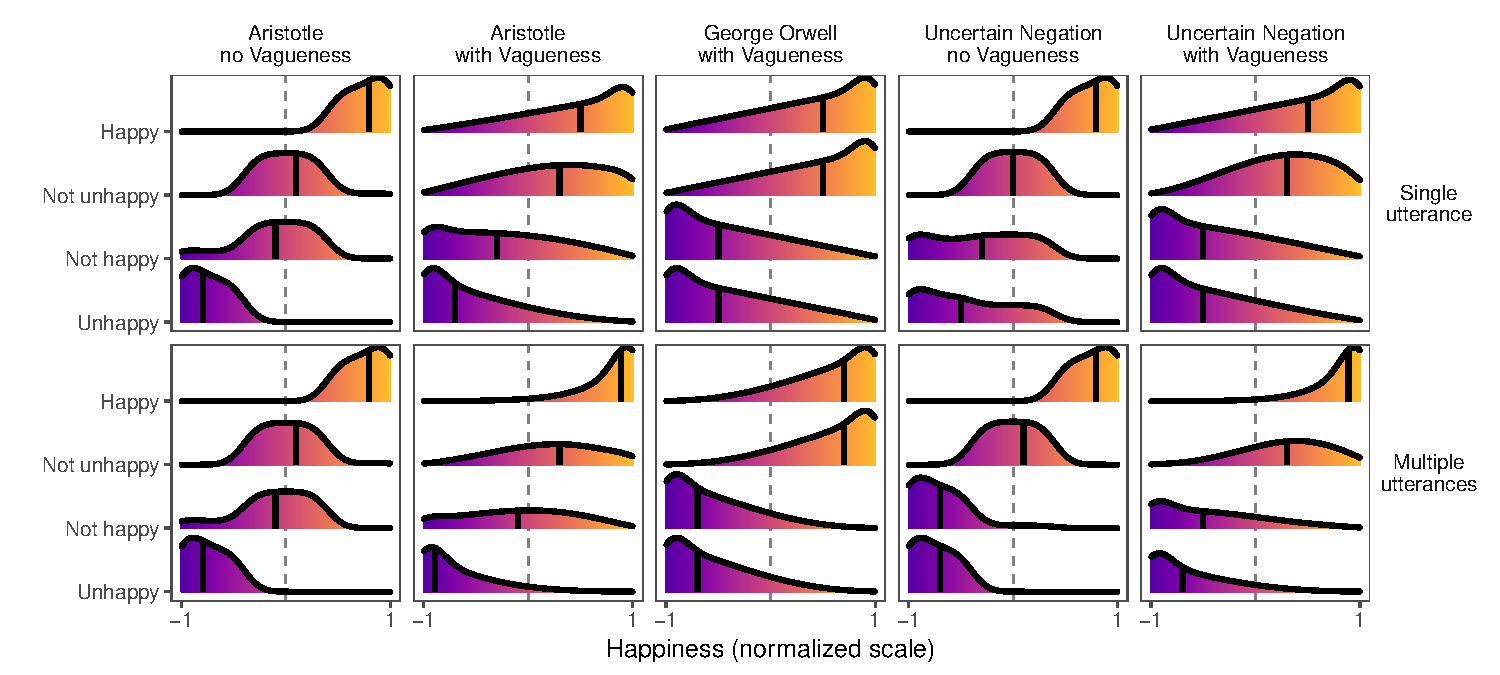
\includegraphics{figs/alternativeModels_all5_dists.pdf} 
\caption{Model predictions for interpretations of antonym pairs and their negations. The \emph{Uncertain Negation} model shows unique qualitative patterns, exhibiting qualities of both the \emph{George Orwell} and \emph{Bonafide Contraries} models when the utterances are presented in isolation (Single Utterance condition); when utterances are presented in the same context (Multiple Utterances condition), \emph{Uncertain Negation} makes predictions similar to the \emph{Bonafide Contraries} model. Model predictions use the following minimally assumptive model parameters: $P(x) = \text{Uniform}(0, 1); \alpha = 1; \text{cost}(\mathit{un}) = 2; \text{cost}(\mathit{not}) = 3$.}.\label{fig:modelPredictions}
\end{figure}
\newpage


% Please add the following required packages to your document preamble:
% \usepackage{booktabs}

%{]}
%--\textgreater{}
A unique pattern of data is predicted by each model.
By design, the \emph{George Orwell} model does not distinguish different kinds of negation, and a double negation like \enquote{not unhappy} returns the same distribution as the positive adjective (\enquote{happy}).
When we hard-code different thresholds for \enquote{happy} and \enquote{unhappy} in the Vanilla RSA model, the model reasons that \enquote{not unhappy} does not communicate the same region of the space as \enquote{happy}; instead, the model restricts its interpretation to the neutral zone (i.e., \emph{not unhappy but not happy}); the same logic plays out for \enquote{not happy}, which receives the same neutral-feelings interpretation. 
The model that represents the vagueness of an adjective like \enquote{happy} and treats \enquote{unhappy} as a \emph{bonafide contrary} predicts the intuitive ordering expressed by \citeA{Krifka2007:Negated-antonyms}: \emph{unhappy} $<$ \emph{not happy} $<$ \emph{not unhappy} $<$ \emph{happy}, with \emph{not unhappy} receiving a slightly positive interpretation.
Finally, the full uncertain negation model predicts a different ordering: The uncertain negation model does not differentiate \enquote{unhappy} (antonyms) from \enquote{not happy} (negated positives), as \citeA{Jespersen1917:Negation} and \citeA{Blutner2004:pragmatics} surmised.
At the same time, upon hearing \enquote{not unhappy}, the \emph{uncertain negation} model reasons that a truly compositional \(\neg \neg \textit{happy}\) is implausible because the speaker could have just said the simpler \enquote{happy} and
interprets the utterance as signaling a slightly positive state (Fig.\(\thinspace\)\ref{fig:modelPredictions}).
%This pattern of judgments is uniquely predicted by the \emph{uncertain negation} model.
%The \emph{bonafide contraries} model also yields interpretations of negated antonyms as slightly positive, but predicts that \enquote{unhappy} (morphological antonym) signals a more negative state than \enquote{not happy} (negated positive).
%The \emph{logical negation} model does not differentiate between negated antonyms and positives, nor between negated positives and antonyms.




The \emph{uncertain negation} model's predictions are derived by reasoning about which lexicon best explains a speaker's utterance (Fig.\(\thinspace\)\ref{fig:modelPredictions}, \emph{single utterance}).
Hearing multiple utterances by the same speaker, however, can provide the listener more information about the speaker's lexicon, as in \citeA{Krifka2007:Negated-antonyms}'s example above (``I wasn't unhappy, just not happy''). 
The formal modeling approach we take here naturally allows for this extension by simply providing \(L_1\) with multiple adjective phrases; we condition each model on the observation of a speaker using all four adjective alternatives to describe different referents (e.g., \enquote{Sue is happy. Steve is not happy. Bill is unhappy. Barb is not unhappy.}; Fig.\(\thinspace\)\ref{fig:modelPredictions}, \emph{multiple utterances}).
Hearing multiple utterances has no effect on the Vanilla RSA model because it ascribes no uncertainty in meaning to the linguistic messages.
The models that do account for the vagueness of predicates derive more extreme differences in interpretations between utterances that could have different meanings (e.g., the difference between ``happy'' and ``not unhappy'' for \emph{Bonafide contraries} is greater when it hears multiple utterances).
This inference results from the fact that the listener has more evidence that the speaker intends different meanings for the different linguistic messages by virtue of the fact that the speaker used different messages.
Crucially, this inference results in the \emph{Uncertain negation} model predicting a meaning difference between \enquote{unhappy} and \enquote{not happy}: \enquote{unhappy} is more sad than \enquote{not happy}, producing the ordering hypothesized by \citeA{Krifka2007:Negated-antonyms} when both are used in the same context.
%All models have more extreme interpretations when they condition on multiple utterances.



%\hypertarget{references}{%
%\section{References}\label{references}%}

\bibliographystyle{apacite}

\setlength{\bibleftmargin}{.125in}
\setlength{\bibindent}{-\bibleftmargin}

\bibliography{negant}

%\begingroup
%\setlength{\parindent}{-0.5in}
%\setlength{\leftskip}{0.5in}
%
%\hypertarget{refs}{}
%\leavevmode\hypertarget{ref-lme4}{}%
%Bates, D., M\wrapmf{\"{a}}chler, M., Bolker, B., \& Walker, S. (2015). Fitting linear mixed-effects models using lme4. \emph{Journal of Statistical Software}, \emph{67}(1), 1--48.
%
%\leavevmode\hypertarget{ref-Bergen2016}{}%
%Bergen, L., Levy, R., \& Goodman, N. D. (2016). Pragmatic reasoning through semantic inference. \emph{Semantics and Pragmatics}, \emph{9}.
%
%\leavevmode\hypertarget{ref-Blutner2004:pragmatics}{}%
%Blutner, R. (2004). Pragmatics and the lexicon. \emph{Handbook of Pragmatics}, \emph{488514}.
%
%\leavevmode\hypertarget{ref-bybee2006usage}{}%
%Bybee, J. L. (2006). From usage to grammar: The mind's response to repetition. \emph{Language}, \emph{82}(4), 711--733.
%
%\leavevmode\hypertarget{ref-Cable2017}{}%
%Cable, S. (2017). The good, the 'not good', and the 'not pretty': Negation in the negative predicates of tlingit.
%
%\leavevmode\hypertarget{ref-Franke2015a}{}%
%Franke, M., \& J\wrapmf{\"{a}}ger, G. (2015). Probabilistic pragmatics, or why Bayes' rule is probably important for pragmatics. In \emph{Zeitschrift für sprachwissenschaft} (pp. 3--44).
%
%\leavevmode\hypertarget{ref-Goodman2016:RSA}{}%
%Goodman, N. D., \& Frank, M. C. (2016). Pragmatic language interpretation as probabilistic inference. \emph{Trends in Cognitive Sciences}, \emph{20}(11), 818--829.
%
%\leavevmode\hypertarget{ref-Horn1989:Natural}{}%
%Horn, L. R. (1989). \emph{A natural history of negation}. University of Chicago Press.
%
%\leavevmode\hypertarget{ref-Horn1991:Duplex}{}%
%Horn, L. R. (1991). Duplex negatio affirmat...: the economy of double negation. \emph{CLS 27-II: Papers from the Parasession on Negation}, 80--106.
%
%\leavevmode\hypertarget{ref-Jespersen1917:Negation}{}%
%Jespersen, O. (1917). \emph{Negation in english and other languages}. Kobenhavn: Host.
%
%\leavevmode\hypertarget{ref-Jespersen1924}{}%
%Jespersen, O. (1924). \emph{The philosophy of grammar}. London: Allen \& Unwin.
%
%\leavevmode\hypertarget{ref-Kennedy2007}{}%
%Kennedy, C. (2007). Vagueness and grammar: the semantics of relative and absolute gradable adjectives. \emph{Linguistics and Philosophy}, \emph{30}, 1--35.
%
%\leavevmode\hypertarget{ref-Krifka2007:Negated-antonyms}{}%
%Krifka, M. (2007). Negated Antonyms: Creating and Filling the Gap. \emph{Presupposition and Implicature in Compositional Semantics}, 163--177.
%
%\leavevmode\hypertarget{ref-Lassiter2015}{}%
%Lassiter, D., \& Goodman, N. D. (2015). Adjectival vagueness in a Bayesian model of interpretation. \emph{Synthese}.
%
%\leavevmode\hypertarget{ref-Markman1989}{}%
%Markman, E. M. (1989). \emph{Categorization and naming in children: Problems of induction}. MIT Press.
%
%\leavevmode\hypertarget{ref-MorganLevy2016:binomials}{}%
%Morgan, E., \& Levy, R. (2016). Abstract knowledge versus direct experience in processing of binomial expressions. \emph{Cognition}, \emph{157}, 384--402.
%
%\leavevmode\hypertarget{ref-Odonnell2015productivity}{}%
%O'Donnell, T. J. (2015). \emph{Productivity and reuse in language: A theory of linguistic computation and storage}. MIT Press.
%
%\leavevmode\hypertarget{ref-Rett2014:eval}{}%
%Rett, J. (2014). \emph{The semantics of evaluativity}. Oxford University Press.
%
%\leavevmode\hypertarget{ref-Yoon2017}{}%
%Yoon, E. J., Tessler, M. H., Goodman, N. D., \& Frank, M. C. (2017). "I won't lie, it wasn't amazing": Modeling polite indirect speech. In \emph{Proceedings of the 39th annual meeting of the cognitive science society}.
%
%\endgroup


\end{document}
